\subsection{Calibration}
%%%%%%%%%%%%%% INTRO %%%%%%%%%%%%%%%

% TODO Elael reler
The hardcoating process currently used considers that the position and
the blade orientation is fixed in relation to the robot and , once correctly that
positioned , the process runs in open loop . However, for any
one of the solutions proposed by this document , you can not assume that neither
position or the orientation of the handler , for the blade to be processed , if
keep fixed.

For a correct path planning the handler must follow during
hardcoating task , it is important knowledge transform between
coordinate system of the manipulator and of the blade being processed . Therefore, it is
must use a system that allows the acquisition of information
respect for the environment and the relative position between the handler and the blades .

%%%%%%%%

O processo de metalização utilizado atualmente considera que a posição e
orientação da pá é fixa em relação ao robô e, uma vez, que corretamente
posicionado, o processo é executado em malha aberta. Entretanto, para qualquer
uma das soluções propostas por esse documento, não é possível assumir que nem a
posição nem a orientação do manipulador, em relação a pá a ser processada, se
manterão fixas.

Para um correto planejamento de trajetória que o manipulador deve seguir durante
a tarefa de metalização, é importante o conhecimento da transformada entre o
sistema de coordenada do manipulador e da pá a ser processada. Portanto, é
necessário utilizar algum sistema que possibilite a aquisição de informações a
respeito do ambiente e da posição relativa entre o manipulador e as pás.

%%%%%%%%%%%%%%%% MKT %%%%%%%%%%%%%%%

\subsection{Estudo de sensores}

A utilização de um sensor de aquisição de dados espaciais não se limita somente
a localização, mas, dependendo do sistema a ser escolhido, pode também ser útil
na reconstrução do modelo do perfil hidráulico da pá, tanto do perfil ideal
quanto do estado atual da pá a ser processada (Tarefas descritas em
\ref{sec::introducao}).

Esta seção irá apresentar os segmentos de sensores que possam suprir essa
necessidade, assim como suas vantagens e limitações. 


\subsubsection{3D scanners}

3D scanners são equipamentos de alta precisão utilizados na indústria
geralmente em aplicações de metrologia, construção civil, monitoramento de
deformações, entre outras. O equipamento consiste em um feixe de laser que é
direcionado por meio de um espelho e a partir da mudança de fase do sinal
refletido é possível calcular a distância até o objeto atingido. O seu preço
esta na faixa de U\$70.000,00.

\paragraph{Estações de medição}

Esse tipo de sensor funciona a partir de um único feixe laser que é direcionado
por um espelho giratório acoplado a um motor de passo de alta resolução. O
sensor possui também uma base giratória, realizando assim um escaneamento de
$360^o$ do ambiente. Graças a sua construção, esse tipo de sensor possui uma
alta densidade de pontos e resolução, porém sua taxa de atualização não é muito
alta.


\begin{center}
\begin{tabular*}{\columnwidth}{l @{\extracolsep{\fill}} cc}
\hline
{\bf Feature}           &
{\bf\begin{tabular}[x]{@{}c@{}}Faro \\Focus X 330\end{tabular}} & {\bf Leica P16}                                               \\ \hline {\bf Complexidade de Software}  & Média                                                      & \cellcolor[HTML]{92D050}{\color[HTML]{000000} {\bf Baixa}} \\
{\bf Custo Material}            & \cellcolor[HTML]{FE0000}{\color[HTML]{FFFFFF} {\bf Alto}}  & Médio                                                      \\
{\bf Tamanho}                   & Grande                                                     & \cellcolor[HTML]{92D050}{\bf Pequeno}                      \\
{\bf Tempo de Resposta}         & \cellcolor[HTML]{FE0000}{\color[HTML]{FFFFFF} {\bf Alto}}  & \cellcolor[HTML]{92D050}{\bf Baixo}                        \\
{\bf Acurácia da Profundidade}  & \cellcolor[HTML]{92D050}{\bf Alta}                         & Média                                                      \\
{\bf Qualidade com Pouca Luz}  & \cellcolor[HTML]{92D050}{\bf Boa}                          & \cellcolor[HTML]{92D050}{\bf Boa}                          \\{\bf Qualidade com Muita Luz} & \cellcolor[HTML]{FE0000}{\color[HTML]{FFFFFF}
{\bf Fraca}} & \cellcolor[HTML]{92D050}{\bf Boa}                          \\
{\bf Consumo de Energia}        & Médio                                                      & \cellcolor[HTML]{92CDDC}{\bf Escalavel}                    \\
{\bf Alcance}                   & \cellcolor[HTML]{92CDDC}{\bf Escalavel}                    & \cellcolor[HTML]{92CDDC}{\bf Escalavel}                    \\ \hline
\end{tabular*}
\captionof{table}{Comparativo Luz Estruturada vs ToF. Fonte: \citep{larrylitof}}
%\caption{Dados principais do processo de metalização HVOF}
\label{tab::estructvstof}
\end{center}

\begin{itemize}
  \item \textbf{Faro Focus X 330}
  	\begin{itemize}
  		\item Campo de visão (vertical/horizontal): $300^o$/$360^o$
  		\item Alcance: 330m
  		\item Velocidade máx. de escaneamento: 976.000pts/s
  		\item Precisão: $\pm$2mm
  		\item Peso: 5,2 kg
  		\item Tamanho: 240 x 200 x 100 mm
  		\item Vida da bateria: 4,5 horas
  		\item Temperatura ambiente: $5^o$ - $40^o$ C
  		\item Preço: U\$70.000,00
	\end{itemize}
  \item \textbf{Leica P16}
  	\begin{itemize}
  		\item Campo de visão (vertical/horizontal): $270^o$/$360^o$
  		\item Alcance: 40m
  		\item Velocidade máx. de escaneamento: 1.000.000pts/s
  		\item Precisão: $\pm$3mm
  		\item Peso: 12,25 kg
  		\item Tamanho: 238 x 358 x 395 mm
  		\item Vida da bateria: 5,5 horas
  		\item Temperatura ambiente: $-20^o$ - $50^o$ C
  		\item Preço: U\$80.000,00
	\end{itemize}
   \item \textbf{Nikon MV330}
  	\begin{itemize}
  		\item Campo de visão (vertical/horizontal): $45^o$/$360^o$
  		\item Alcance: 30m
  		\item Velocidade máx. de escaneamento: 2000pts/s
  		\item Precisão: $\pm$0.5mm
  		\item Peso: \textit{não informado}
  		\item Tamanho: \textit{não informado}
  		\item Vida da bateria: \textit{não informado}
  		\item Temperatura ambiente: \textit{não informado}
  		\item Preço: U\$355.000,00
	\end{itemize}


\end{itemize}


\begin{figure}[h!]
	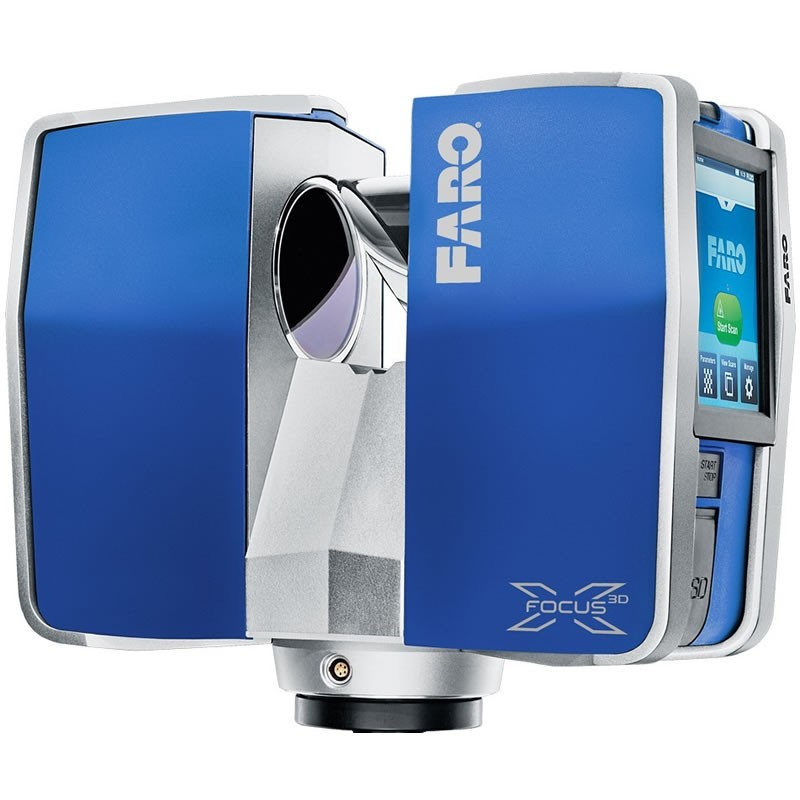
\includegraphics[width=0.6\columnwidth]{figs/3dsensors/faro}
	\caption{Sensor Faro Focus X330}
    \label{fig::faro_focus}
\end{figure}

%TODO acertar figura

\paragraph{Velodyne}

A empresa Velodyne possui, atualmente, 3 modelos de 3D Lidar. Os modelos variam
basicamente no número de pares de emissores e receptores e, consequentemente, na
resolução final. Os modelos são o VLP-16, o HDL-32E e HDL-64E, com 16,32 e 64
canais respectivamente. Esse tipo de sensor possui uma alta taxa de
atualização, entretanto não possui uma alta densidade de dados. O modelo mais
utilizado é o intermediário HDL-32E.

\begin{itemize}
\item 32 pares laser/detector  
\item Campo de Visão: +10.67$^o$ to -30.67$^o$ (vertical)
\item Rotação de $360^o$
\item Alcance - 1m - 100m 
\item 10 Hz frame rate (selecionável 5-20Hz)
\item Temperatura de Operação $-10^o$ to $+60^o$ C
\item Acurácia: $<$2 cm
\item Resolução Angular (vertical) 1.33$^o$
\item Peso: HDL-32E = 1kg; Cabos = 0.3kg
\item Tamanho: 15cm altura x 8.6cm diâmetro
\item Proteção: IP67
\item Correção de orientação (internal MEMS acelerometros and gyros)
\end{itemize}

\begin{figure}[h!]
   \centering
   \includegraphics[width=0.8\columnwidth]{figs/3dsensors/velodyne}
   \caption{Velodyne Models}
   \label{fig::velodyne_models}
\end{figure}

\paragraph{Forecast 3D Laser System}


O sensor Forecast 3D consiste em um senor 2D laser da SICK, modelo LMS 151 ou
511, acoplado a uma unidade $pan-tilt$. O seu preço esta na faixa de
U\$37.000,00.


\begin{figure}[h!]
   \centering
   \includegraphics[width=0.8\columnwidth]{figs/3dsensors/forecast}
   \caption{Forecast 3D Laser System}
   \label{fig::forecast}
\end{figure}

\subsubsection{ToF Cameras}

Conhecidas como Time-of-Flight Cameras, são dispositivos compostos por apenas
uma câmera, não necessitando de uma configuração estéreo para triangularização
de imagens. Esse tipo de dispositivo utiliza uma fonte infra-vermelho interna e de
forma análoga aos dispositivos laser, calcula a distância a partir da diferença
de fase do sinal refletido. Entretanto, essa tecnologia possibilita o cálculo
simultâneo das distâncias de cada objeto na região iluminada pela fonte IR,
mesmo que com resoluções limitadas.

\paragraph{Mesa Imaging SwissRanger SR4000}


\begin{itemize}
  \item Alcance para detecção: 0.1 - 10.0 m
  \item Alcance calibrado: 0.8 - 8.0 m
  \item Drift com a temperatura (T) - $\leq$ 1.5 mm/$^o$C (max.) - For 10$^o$C
  $\leq$ T $\leq$ 50$^o$C
  \item Tamanho: 65 x 65 x 76 mm
  \item Peso: 510 g
\end{itemize}

\begin{figure}[h!]
   \centering
   \includegraphics[width=0.8\columnwidth]{figs/3dsensors/mesa2}
   \caption{Mesa Imaging SwissRanger SR4000}
   \label{fig::mesa}
\end{figure}

\paragraph{Sentis M100 / Argos 3D - P100}

\begin{itemize}
  \item Medidas de distância e vídeo em tons de cinza
  \item Resolução: 160 x 120 pixels
  \item 40 - 160 fps
  \item Alcance: $>$3m  (extensível até 10m indoor)
  \item Campo de Visão: $90^o$
  \item Tamanho: 75 x 57 x 26 mm
  \item Peso:
\end{itemize}

\begin{figure}[h!]
   \centering
   \includegraphics[width=0.8\columnwidth]{figs/3dsensors/argos3dp100}
   \caption{Sensor Argos 3D - P100}
   \label{fig::forecast}
\end{figure}

\subsubsection{Câmeras de Luz Estruturada}

Estes sensores constituem de uma fonte emissora de infra-vermelho e um receptor.
Um padrão é projetado na cena a ser reconstruida e a partir da distorção desse
padrão é possível o cálculo de distâncias. 

%TODO exemplos dos sensores de luz estruturada
%TODO Pros e cons

%TODO ELAEL - decidir se abre uma subseção d eaplicações ou coloca um exemplo de
% aplicação em cada componente - utilizar o seu material do SOTA em 3D sensors. 

\begin{center}
\begin{tabular*}{\columnwidth}{l @{\extracolsep{\fill}} cc}
\hline
{\bf Características}           &
{\bf\begin{tabular}[x]{@{}c@{}}Luz\\Estruturada\end{tabular}} & {\bf ToF}                                               \\ \hline {\bf Complexidade de Software}  & Média                                                      & \cellcolor[HTML]{92D050}{\color[HTML]{000000} {\bf Baixa}} \\
{\bf Custo Material}            & \cellcolor[HTML]{FE0000}{\color[HTML]{FFFFFF} {\bf Alto}}  & Médio                                                      \\
{\bf Tamanho}                   & Grande                                                     & \cellcolor[HTML]{92D050}{\bf Pequeno}                      \\
{\bf Tempo de Resposta}         & \cellcolor[HTML]{FE0000}{\color[HTML]{FFFFFF} {\bf Alto}}  & \cellcolor[HTML]{92D050}{\bf Baixo}                        \\
{\bf Acurácia da Profundidade}  & \cellcolor[HTML]{92D050}{\bf Alta}                         & Média                                                      \\
{\bf Qualidade com Pouca Luz}  & \cellcolor[HTML]{92D050}{\bf Boa}                          & \cellcolor[HTML]{92D050}{\bf Boa}                          \\{\bf Qualidade com Muita Luz} & \cellcolor[HTML]{FE0000}{\color[HTML]{FFFFFF}
{\bf Fraca}} & \cellcolor[HTML]{92D050}{\bf Boa}                          \\
{\bf Consumo de Energia}        & Médio                                                      & \cellcolor[HTML]{92CDDC}{\bf Escalavel}                    \\
{\bf Alcance}                   & \cellcolor[HTML]{92CDDC}{\bf Escalavel}                    & \cellcolor[HTML]{92CDDC}{\bf Escalavel}                    \\ \hline
\end{tabular*}
\captionof{table}{Comparativo Luz Estruturada vs ToF. Fonte: \citep{larrylitof}}
%\caption{Dados principais do processo de metalização HVOF}
\label{tab::estructvstof}
\end{center}

\subsection{Conclusão}

As restrições apresentadas pelo problema de calibração, dentro do ambiente da
turbina, impõem um conjunto de requisitos mínimos que o sensor deve apresentar:

\begin{itemize}
  \item Alta resolução
  \item Portabilidade
  \item Alcance suficiente (>20m)
  \item Resistir as condições de temperatura e umidade 
\end{itemize}

Além desses requisitos, é desejável também que o sensor tenha alimentação
idependente e que sua velocidade de escaneamento não seja um fator limitante
para a eficiência do processo.

A classe de sensores que atende todas essas condições é a das Estações de
medição, com exceção do sensor Nikon MV 330 que não possui a portabilidade
necessária para a solução proposta, além de ter um preço muito maior que de seus
concorrentes.

O sensor Faro Focus X330, além de satisfazer os requisitos mínimos, é o que
possui menor preço e, por isso, foi escolhido como o o sensor a ser utilizado na
calibração do sistema e reponsável por colher os dados espacias do ambiente da
turbina e do robô. 

Entretanto, pelas especificações do sistema não foi possível garantir a perfeita
operação do sensor nas condições de alta umidade apresentada no interior da
turbina. O dipositivo opera com um sistema de lentes e lasers e, caso apresente
condensação em um desses componentes, o resultado final de sensoriamento pode
ser prejudicado. Devido a este fato, foi realizado uma bateria de testes na
Usina de Jirau, no interior de uma turbina, afim de confirmar a viabilidade
técnica desse sensor.

O teste realizado constituiu na utlização de quatro esferas reflexivas,
representadas na figura \ref{fig::esferas}, distribuidas pelo ambiente da
turbina.
Em seguida, foram realizadas 4 coletas de dados, sendo 3 delas à jusante do
rotor e uma entre as pás do rotor e o distribuidor. Com a nuvem de pontos
coletada, foi possível utilizar a assinatura única gerada pelas esferas para
alinhar todos os conjuntos de dados em uma única imagem 3D.

\begin{figure}[h!]
\centering
	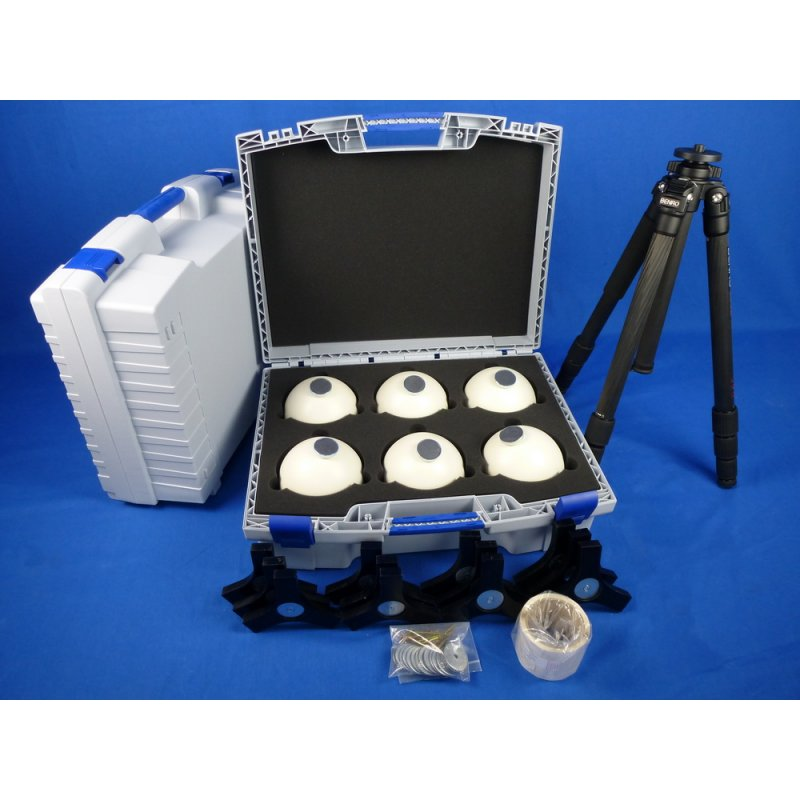
\includegraphics[width=0.9\columnwidth]{figs/3dsensors/kit}
	\caption{Conjunto de esferas reflexivas e tripé}
	\label{fig::esferas}
\end{figure}

A figura \ref{fig::turbina_faro} representa a vista frontal da imagem gerada e, por sua
vez, a figura \ref{fig::turbina_cad} representa uma reconstrução 3D gerada a
partir da nuvem de pontos coletas e utilizando o software proprietário do
fornecedor do sensor. 

\begin{figure}[h!]
\centering
	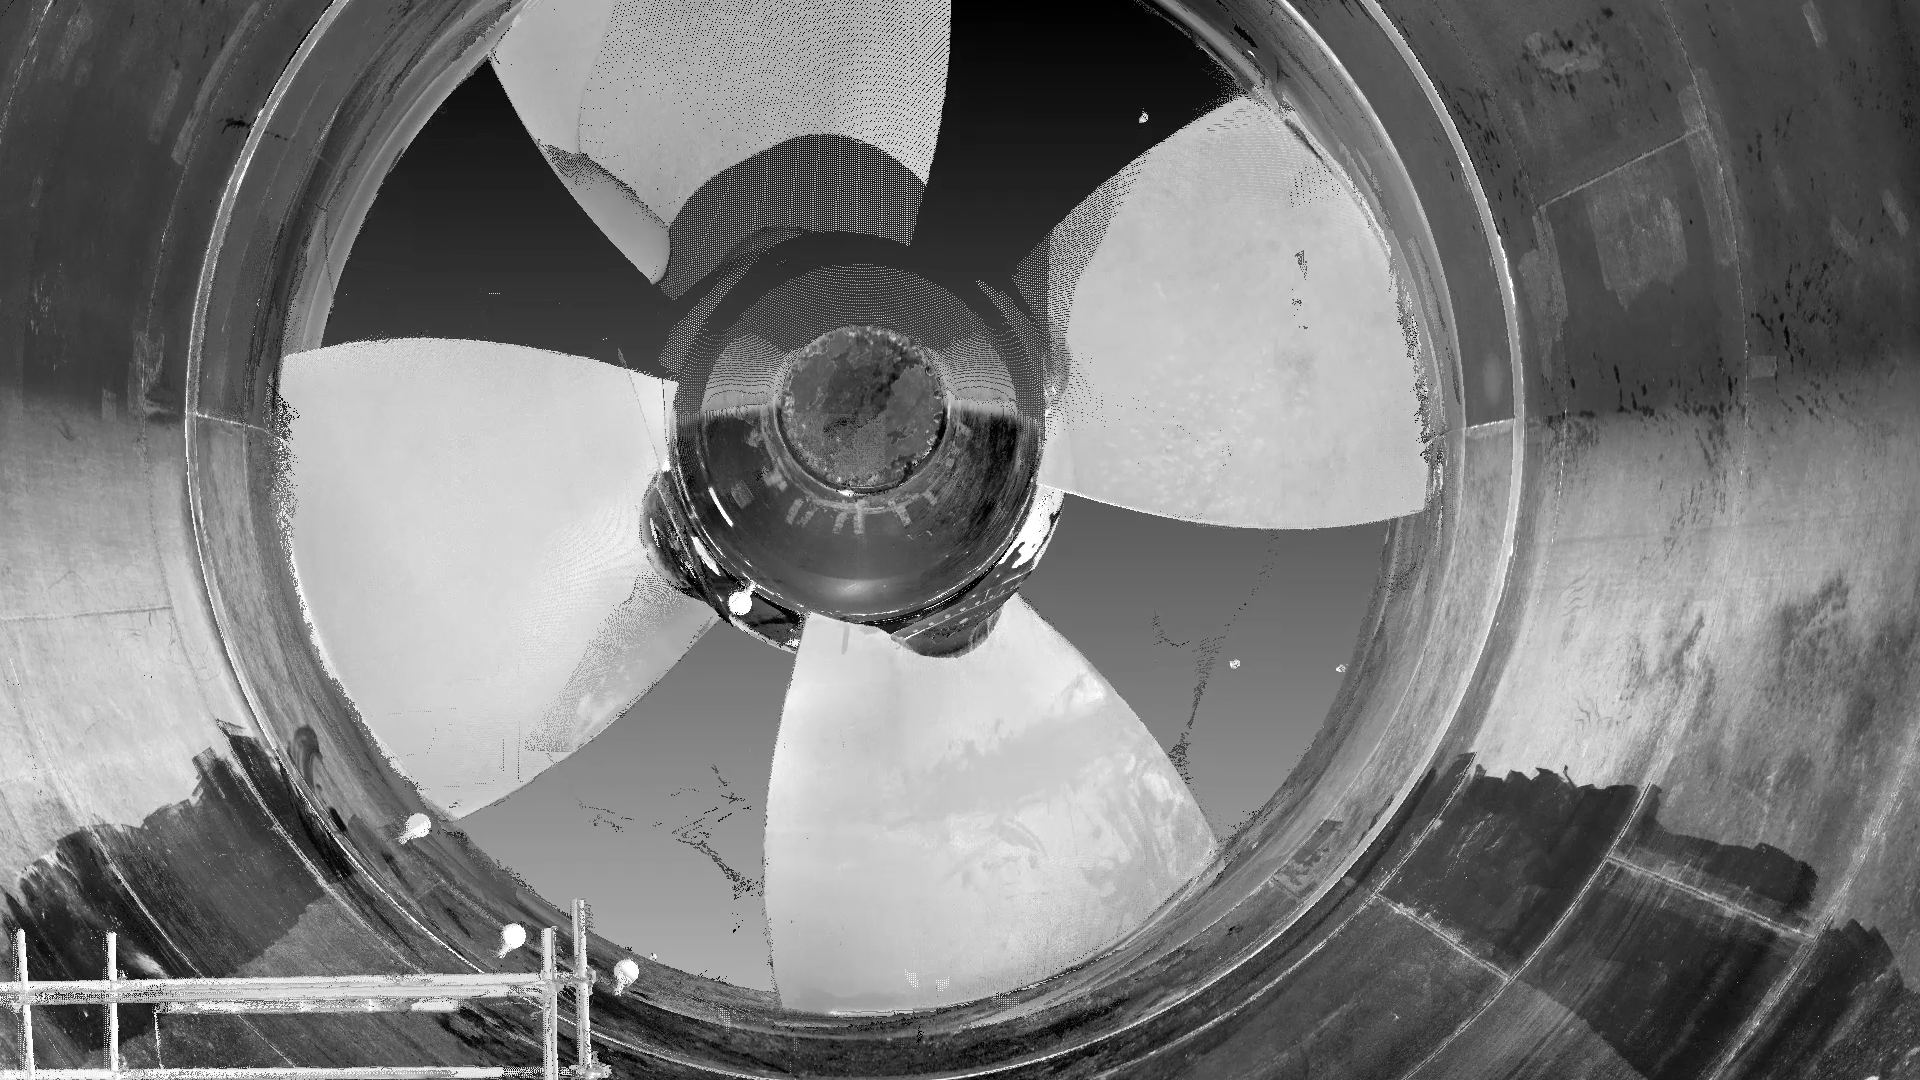
\includegraphics[width=0.9\columnwidth]{figs/3dsensors/recorte_video}
	\caption{Vista frontal da imagem gerada a partir dados adquiridos durante o
	teste.}
	\label{fig::turbina_faro}
\end{figure}

\begin{figure}[h!]
\centering
	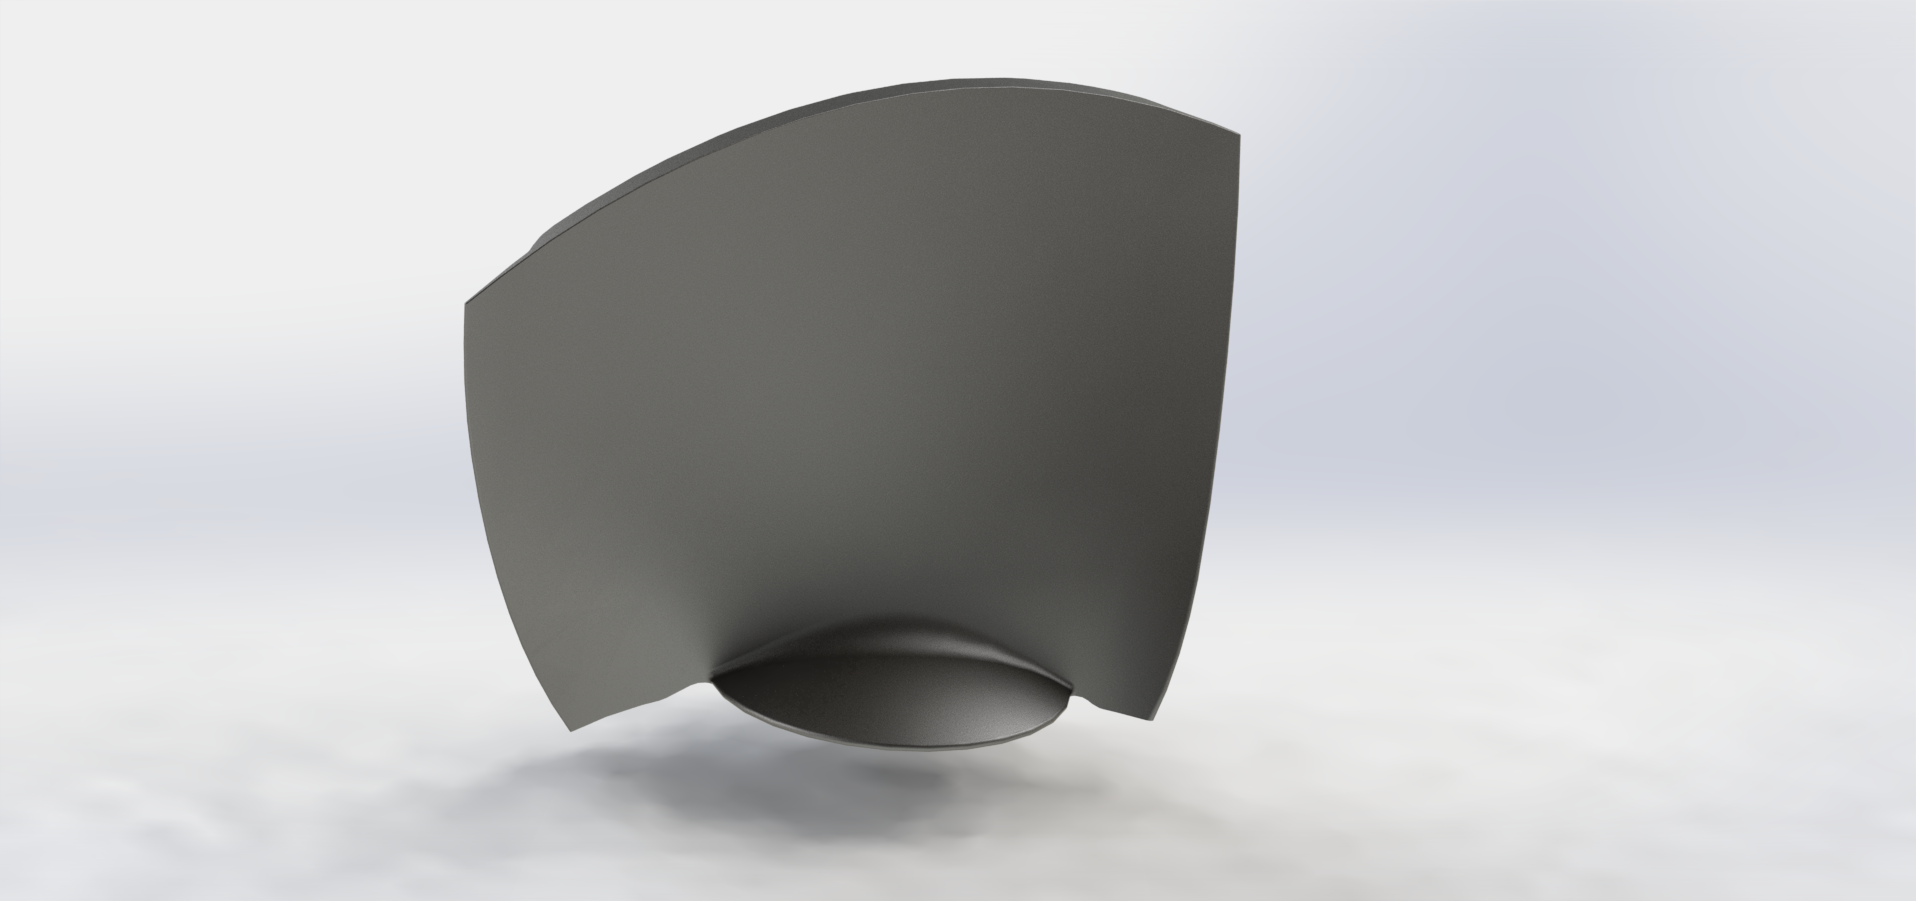
\includegraphics[width=0.9\columnwidth]{figs/3dsensors/Pa_Real_Render_04}
	\caption{Reconstrução em CAD da pá com os dados do teste.}
	\label{fig::turbina_cad}
\end{figure}

A partir dos resultados gerados durante os testes foi comprovada que o sensor é
capaz de operar nas condições extremas impostas pela turbina e com um nível de
ruído aceitável para a aplicação em questão. 


\subsubsection{Medidor de distância a Laser}

Durante o processo de metalização o 3D scanner estará desligado, pois o tempo de
varedura não o torna prático para obter informações em tempo real. Assim o
sistema estaria funcionando em \textit{loop} aberto, o que gera receios com
relação à segurança. A fim de evitar tais riscos é desejável alguma
realimentação para o sistema sobre sua posição. Essa realimentação será
realizada pelo uso de um medidor de distância a Laser, a ser posicionado próximo
à pistola de metalização, com o intuito de aferir a distância da pistola até a
pá em tempo real.

\begin{figure}[h!]
\centering
	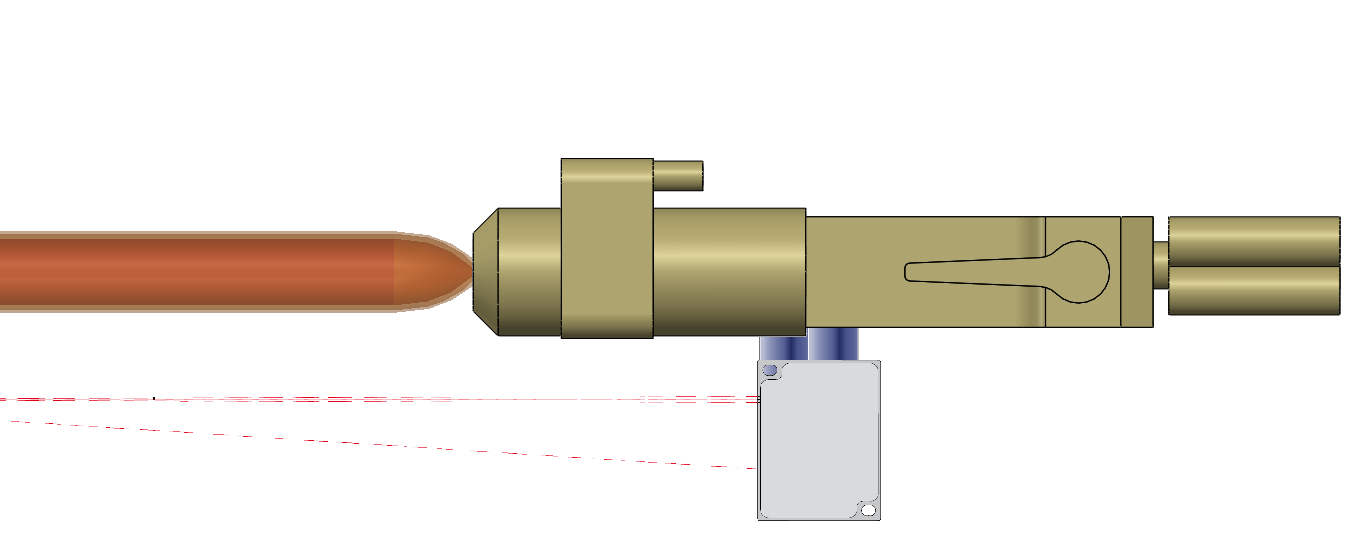
\includegraphics[width=0.9\columnwidth]{figs/3dsensors/senso_laser_pistola}
	\caption{Ilustração da posição do medidor de distância, em cinza, na pistola de
	metalização.}
	\label{fig::laser}
\end{figure}


Para a escolha de medidor compatível foram analisadas as seguintes variáveis:

\paragraph{Temperatura}
A temperatura da superfície pode influenciar na precisão do sensor devido à
radiação de corpo negro. Caso essa radiação térmica atinja níveis relevantes na
faixa de frequência do Laser utilizado ocorre degradação da qualidade de
reposta do sensor. Análises de campo identificaram que, apesar da alta
temperatura da chama de metalização, a pá da turbina não chega a emitir níveis
preocupantes de radiação na faixa do vermelho ($670 nm$), onde operam os Lasers
padrões. Para casos de exceção existem Laser que trabalham em regiões do
azul/violeta.

Por outro lado a temperatura do ambiente também influencia o sensor, que não
costuma ter alta resistência à temperatura, ficando algo em torno do $50^oC$.
Para evitar que o calor da chama seja recebido diretamente pelo sensor,
aumentando a temperatura ambiente na região, ele deve ser posicionado na pistola
com uma distância de segurança da chama (figura \ref{fig::laser}).

\paragraph{Distância de operação}
A metalização ocorre com a pistola entre 23cm e 24cm de distância da pá. Somado
a isso temos a distância do sensor à chama para então sabermos a distância da
pá ao sensor. Considerando que a pistola possui em torno de 30cm de comprimento,
a faixa de operação de distâncias do sensor deverá incluir 40-50cm. Para termos
essa região no centro da faixa de operação, ela deverá iniciar em 20-25cm e
trabalhar até 80-100cm.

\paragraph{Poeira e Umidade}
A alta umidade ambiente dentro do aro câmara, e em todo circuito hidráulico,
impõe mais um requisto sobre o equipamento. Além disso, o pó residual da
aplicação da metalização pode ser danoso ao sensor. Um isolamento apropriado
para o sensor pode ser encontrado segundo a padronização IP69K.

\paragraph{Precisão}
Como a tolerância está na ordem de milímetros ( a distância do sensor à pá deve
se manter em uma faixa de $\pm 5mm $ entre 23cm e 24cm ), logo é desejável que o
sensor possua precisão de $1mm$ ou menor.

\paragraph{Peso}
Considerando a carga máxima no punho do robô de 10kg, e a massa da pistola de
8,5kg e aplicando as restrições dinâmicas ( para manter a velocidade
desejada em todos os pontos ) conclui-se que o medido deve ter uma massa
inferior a 1kg.

%%%%%%%%%%%%%%%  TECNICAS %%%%%%%%%%%%%%%%%%%%%%

\subsection{Estudo de técnicas de reconhecimento} 

As informações de distância recebidas pelos sensores descritos na seção
anterior podem ser armazenados como uma estrutura de dados chamada nuvem de
pontos, isto é, uma representação tridimensional do espaço cartesiano, na qual cada distância medida pelos
sensores a partir de sua origem representa uma coordenada x y z.
Entretanto, essa representação não é capaz de diferenciar, ou classificar, os
limites de cada objeto presente na cena, ou seja, não é possível determinar
\textit{a priori} qual conjunto de pontos pertence a cada elemento que se deseja
identificar para realizar a calibração.

A identificação de cada conjunto, ou \textit{cluster}, de pontos é importante
para que a posição e orientação de cada objeto de interesse seja determinada e,
assim a transformação do sistema de coordenadas entre cada objeto seja
calculada. Esse processo necessita, então, do estudo e implementação de
algoritmos para a análise da nuvem de pontos, identificação dos elementos
necessários, extração de suas respectivas posições e, finalmente, cálculo da
transformação entre as posições. 

Dependendo das características de cada objeto a ser identificado e da
possibilidade de implementação de uma estrutura de apoio para facilitar a sua
identificação, podem ser utilizados diferentes métodos e estratégias de
identificação e localização, que serão exploradas a seguir.

\subsubsection{Reconhecimento do Robô}

O Robô é uma estrutura que a idenficação pode ser facilitada pelo uso de
padrões de fácil reconhecimento (como esferas e padrões de xadrez, figuras
\ref{fig::sphere_rec} e \ref{fig::checkerboard_rec} ), pois alterações na base
do robô não ocasionam problemas para o funcionamento do sistema.


\begin{figure}[h!]
   \centering
   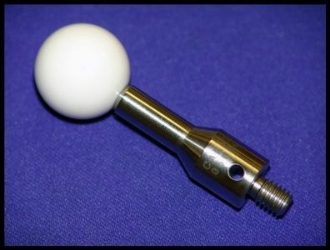
\includegraphics[width=0.95\columnwidth]{figs/localizacao/sphere_rec}
   \caption{Exemplo de esfera utilizada para reconhecimento. Fonte:
   http://shop.talwin.net/}
   \label{fig::sphere_rec}
\end{figure}



\begin{figure}[h!]
   \centering
   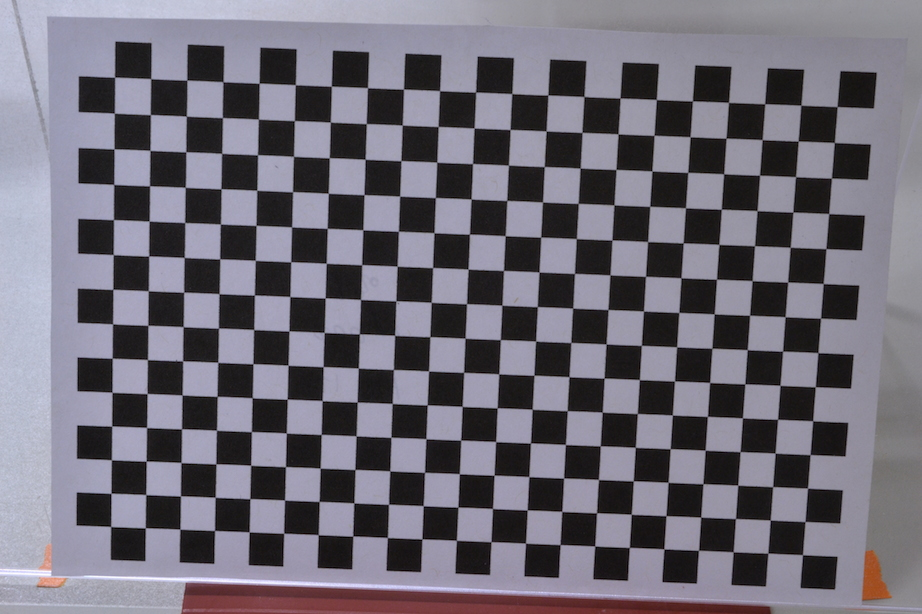
\includegraphics[width=0.95\columnwidth]{figs/localizacao/checkerboard_rec}
   \caption{Exemplo de padrão de xadrez utilizado para renhecimento.\\ Fonte:
   http://stereomorph.blogspot.com.br/}
   \label{fig::checkerboard_rec}
\end{figure}


Devido a baixa iluminação ambiente dentro do circui\-to da tubina, a opção
mais simples é o uso de nu\-vem de pontos sem identificação de cor. Ou seja, o
reconhecimento se dará apenas pelo formato. Isso restringe o uso de padrões de
xadrez e o foco se voltará, então, para o uso de formatos geométricos. Em
especial o mais simples objeto de três dimensões: a esfera.

O reconhecimento de formas geométricas simples em três dimensões é um assunto
já razoavelmente explorado na literatura. Dentre eles pode-se destacar 2
métodos: RANSAC e Hough Transform.

\paragraph{RANSAC}
O método RANSAC (acrônimo para ``RANdom SAmple Consensus", \textit{consenso por
amostragem aleatória} em tradução livre) é um método iterativo que tem como
premissa a presença de \textit{outliers} (elementos fora do corpo principal) na
amostra e objetiva a identificação dos parâmetros matemáticos que descrevem o
objeto geométrico em questão \cite{ransac}. É o método
disponível na amplamente utilizada biblioteca de processamento de nuvem de pontos ``PCL''. 

Esse método consiste na seleção aleatória de pontos para serem considerados como
partes integrantes do corpo principal (no caso, uma esfera), a partir desses os
parâmetros da esfera são calculados (comumente, os valores x, y e z do centro
da esfera e seu raio). Então os demais pontos são julgados como fazendo parte ou
não da esfera de acordo com esses parâmetros. O modelo é avaliado como bem estimado se uma quantidade razoável de pontos são considerados
como pertencentes à esfera. Se for visto como bem estimado, os parâmetros são
então reestimado levando em conta de todos os pontos que foram considerados como
pertencentes à esfera. O erro do modelo é inferido a partir dos pontos que foram
considerados como fazendo parte da esfera e uma esfera reconstruída pelos
parâmetros calculados. O processo então é repetido um número artrário de vezes,
e se mantém armazenado o modelo que obteve menor erro.

Um dos principais pontos negativos do RANSAC é que ele tem como premissa a
presença de apenas um corpo principal, ou seja, apenas uma esfera. Isso implica
em um tratamento especial quando temos mais de uma esfera no ambiente.

\begin{figure}[h!]
   \centering
   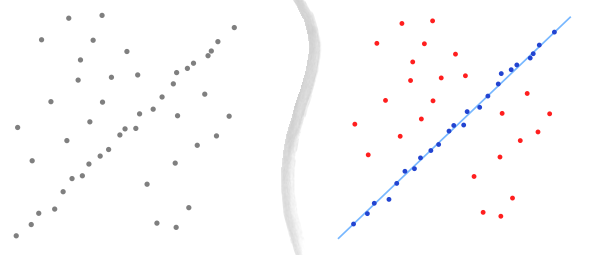
\includegraphics[width=0.95\columnwidth]{figs/localizacao/ransac}
   \caption{Exemplo de reconhecimento de uma linha em 2 dimensões usando
   RANSAC. (Fonte: \cite{ransac})}
   \label{fig::ransac}
\end{figure}
 
 \paragraph{Transformada de Hough 3D}
Anos de pesquisa em reconhecimento de objetos geométricos de duas dimensões
levaram ao desenvolvimento e aprimoramento de técnicas basedas em ``Transformada
de Hough''. Essas técnicas tem sido recentemente adaptadas para o universo de
três dimensões (ver \cite{hough2014}) e adequadamente chamadas de Transformada
de Hough 3D.

O método consiste em tranformar cada ponto do espaço 3D em uma variedade
mergulhada no espaço quadridimensional dos parâmetros da esfera ( x, y e z do
centro mais r do raio). A variedade se identifica com todas as possiveis esferas
que contém aquele ponto. O espaço de parâmetros é então restrito dentro de
certos limites e quantizado por razões de implementação (os recursos
computacionais são finitos). É definido então um acumulador, basicamente uma
função que conta quantas variedade interceptam determinada região discretizada
do espaço de parâmetros. Um algorítmo de reconhecimento de picos é aplicado
sobre o espaço de parâmetros (com as varidade já mergulhadas nele) para detectar
qual o conjunto de parâmetros que está melhor descrevendo um maior número de
pontos. O algorítmo pode ser utilizado para reconhecer mais de um pico e, assim,
identificar a presença de mais de uma esfera na nuvem de pontos (exemplo na
figura \ref{fig::hough}).

A dificuldade no uso do método é seu custo computacional, mas existem soluções
que exploram amostragens estatísticas para reduzir o custo computacional.

\begin{figure}[h!]
   \centering
   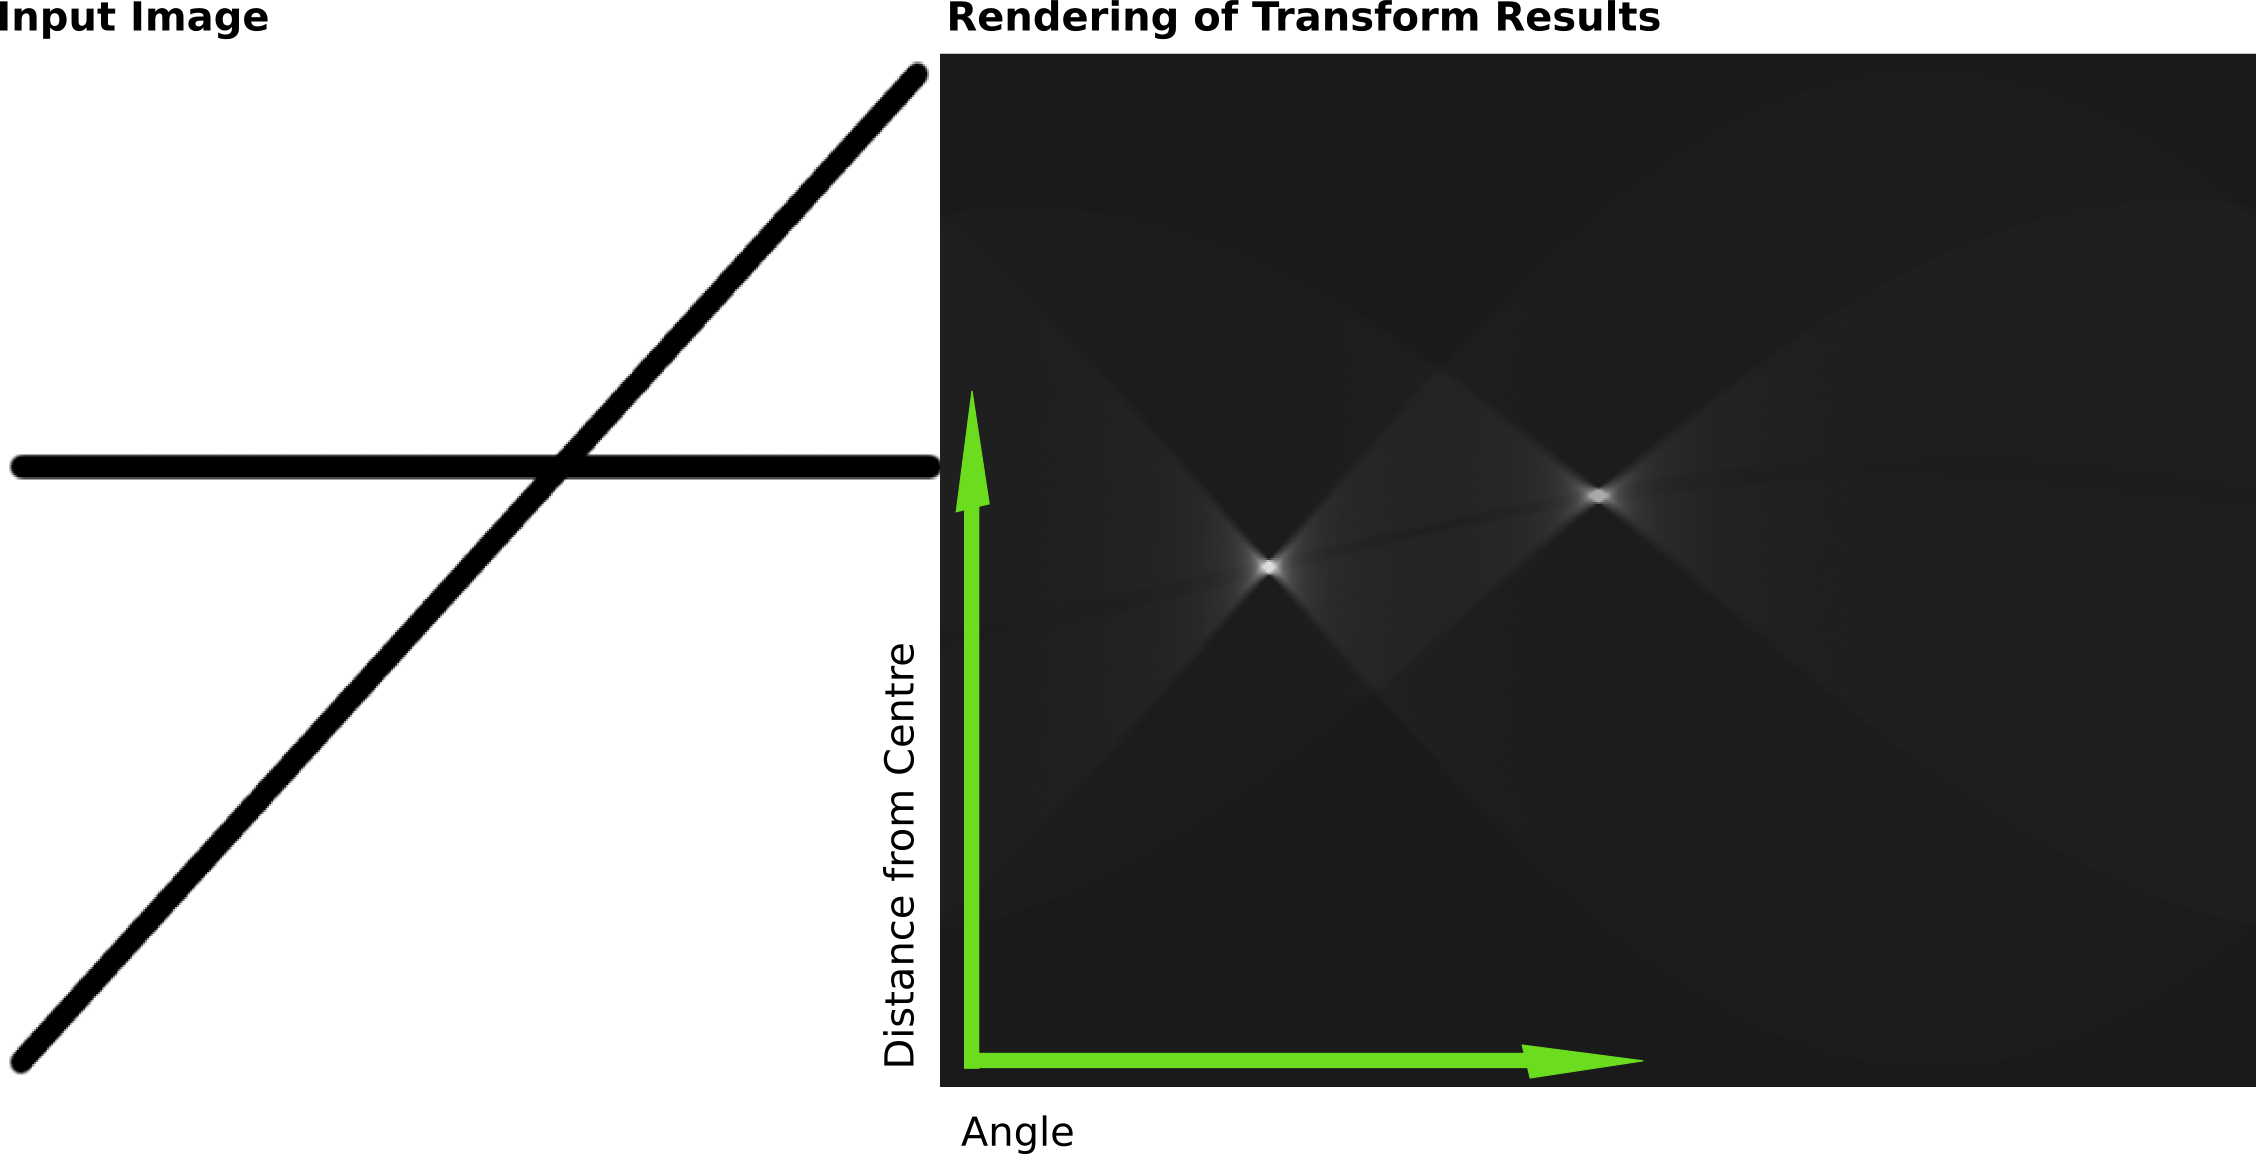
\includegraphics[width=0.95\columnwidth]{figs/localizacao/hough}
   \caption{Exemplo de reconhecimento de duas linhas em 2 dimensões usando
   Transformada de Hough. Na esquerda estão pontos que compõem as duas retas, na
   direita uma sobreposição das variedades referentes a cada ponto das retas
   (mergulhadas em um espaço paramétrico bidimensional). Os pontos mais
   brilhantes refletem os picos referentes aos parâmetros que melhor descrevem as duas retas. (Fonte: 
   \url{https://en.wikipedia.org/wiki/Hough_transform})}
   \label{fig::hough}
\end{figure}

Tendo conhecimento da posição de quatro esferas, pelo uso de um dos métodos
descritos acima, é possivel unicamente identificar a posição de um corpo preso a
elas. Em outras palavras, consegue-se a transformada entre origem do sistema de
coordenadas (tipicamente no sensor) e o robô. Para descobrir a trasnformada
entre o robô e a pá (posição relativa entre eles) falta identificar a
transformada entre a origem e a pá, esse caso será explorado na próxima seção a
seguir.

\subsubsection{Reconhecimento da Pá} 

Para a identificação e localização das pás das turbinas não é possível a
utilização de nenhum artifício de apoio que facilite o processamento da nuvem de
pontos, pois a instalação de qualquer um desses aparatos não pode ter precisão
garantida nas operações de campo. Uma instalação de um elemento de apoio em
pontos precisos da pá necessitaria também de calibração para cada utilização, retirando assim
o propósito do método. 

Portanto, para a localização das pás da turbina é
necessário explorar as características espaciais intrínsecas à superfície do
próprio objeto e identificá-las na nuvem de pontos do ambiente. O objetivo
principal nessa etapa do processo é, então, identificar um conjunto mínimo de
características do objeto que o represente unicamente com um baixo grau
de ambiguidade e sem exigir muito esforço computacional. 

A escolha do tipo de característica a se usar é uma decisão fundamental para a
eficiência do processo e tem sido alvo de estudos na literatura para a análise
e reconhecimento de imagens 2D, como imagens RGB de câmeras e mais recentemente
também para imagens 3D. 

Uma boa representação de \textit{point feature} deve ser capaz de capturar as
mesmas características locais da superfície na presença de:

\begin{itemize}
  \item \textbf{Transformadas} -  rotações e translações 3D nos dados não devem
  influenciar a estimação dos descriptors;
  \item \textbf{Variações na densidade de amostragem} - em princípio, uma de
  superfície amostrada mais ou menos densamente deve ter a mesma assinatura característica do vetor
  \item \textbf{Ruído}
\end{itemize}

O reconhecimento de objetos em aplicações robóticas também vem recebido
grande atenção, principamente com o crescimento da robótica móvel e em ambientes
não estruturados, onde é necessário identificar e localizar os objetos a serem
manipulados em cada tarefa. O problema é enfrentado basicamente utilizando-se
duas abordagens: analisar os dados 3D ou realizar algum tipo de processamento e
projeção para se trabalhar com imagens 2D e utilizar as técnicas mais maduras
desse tipo de imagem.

Nesta última categoria, a técnica
mais usada consiste em converter as informações tridimensionais em \textit{Range
Images}, na qual é realizada uma projeção a partir de um ponto de vista (geralmente o do sensor) e utiliza escala
de cores ou cinza para representar a distância, ou seja, quanto mais escuro o
objeto na imagem, mais longe ele se encontra. É importante reassaltar que esse
tipo de método introduz perdas de informação ao se realizar projeções e é
sensível à escolha do ponto de vista escolhido. 
%Em \cite{Bayramoglu2010} são
%utilizados descritores SIFT, ou \textit{Scale-Invariant Feature Transform},  
%como características a serem identificadas na imagem. \textit{Local Feature
%Histograms} são utilizados em \cite{Hetzel2001} e por sua vez \cite{Chen2007}
%optou por utilizar \textit{Local surface patches}. 
A escolha do descritor a ser
utilizado depende da aplicação e deve ser estudada a melhor opção para a nossa
solução, assim que tivermos dados aquisitados pelo sensor. Aplicações
semelhantes envolvendo identificação de objetos no ambiente tridimensional, mas
sem localizá-los, e utilizando diferentes descritores podem ser encotradas em
\cite{Bayramoglu2010,Hetzel2001,Chen2007}. Uma comparação dos descritores
utilizados para reconhecimento de objetos 2D e 3D pode ser encontrado em \cite{Zaharia2004, Weber2014}.

Após o reconhecimento do objeto, é necessário identificar a sua posição.
Em \cite{Steder2009}, o alinhamento é realizado utilizando-se a própria
\textit{Range Image} e a informação de profundidade presente na mesma. Por outro
lado, em \cite{Nuchter2005} a região onde o objeto identificado está presente é
selecionada e, por meio de \textit{raycasting} o conjunto de pontos da nuvem
pertecentes à região identificada na \textit{Range Image} é reprojetado. Após
essa segmentação, é utilizado um algoritmo de alinhamento como o ICP.

O primeiro passo para tornar possível a localização da pá é a aquisição de seus
dados espacias e a criação de uma nuvem de pontos que a represente. A
figura \ref{fig::pa_pcd} ilustra uma nuvem de pontos representando uma pá de uma das
turbinas da usina de Jirau, esse modelo foi construído utilizando-se os dados
aquisitados durante a viagem de campo e teste de sensibilidade do sensor Faro
Focus X330, como citado anteriormente. É importante ressaltar que o
modelo deve representar, se possível, todas as características pertinentes do objeto de interesse. Nesse
sentido, se faz necessário a criação de um modelo para cada tipo de pá que
deverá ser processada, ou seja pás com diferentes perfis hidráulicos possuem
modelos diferentes.


\begin{figure}[h!]
   \centering
   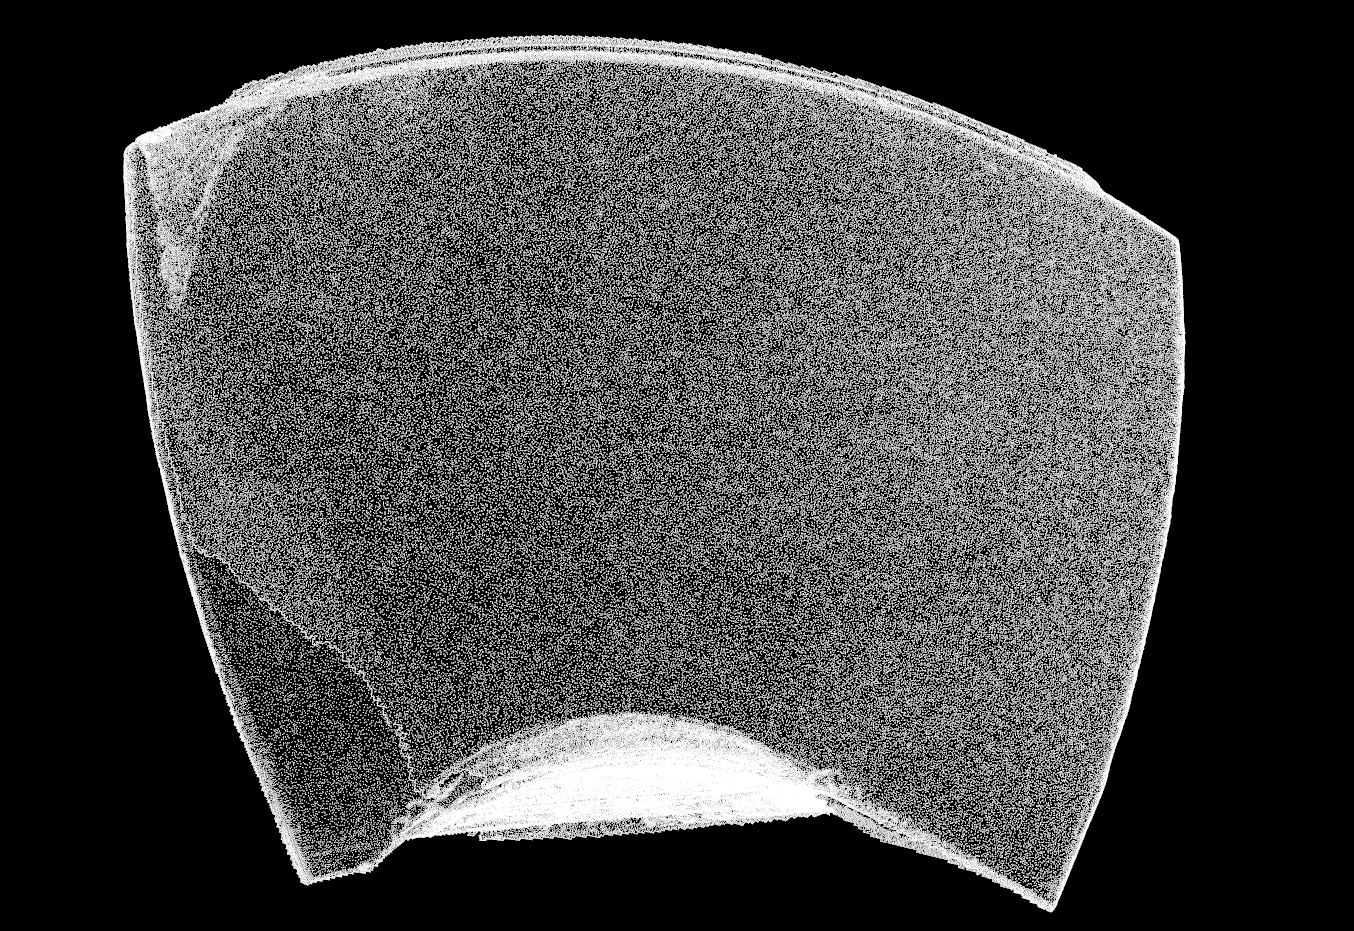
\includegraphics[width=0.95\columnwidth]{figs/localizacao/pa_pcd}
   \caption{Modelo da pá em nuvem de pontos}
   \label{fig::pa_pcd}
\end{figure}

A partir do modelo, é necessário a extração de seus pontos chaves e descritores.
A figura \ref{fig::pa_key} ilustra descritores do tipo SHOT, identificados no modelo de referência da pá. Para a nossa aplicação, não é
necessário, a princípio, o reconhecimento do objeto em questão, apenas a sua
localização e orientação no espaço tridimensional. A possibilidade de inserir no
sistema a informação de qual modelo de pá deve ser procurado, simplifica o
algoritmo e o torna menos suscetível a erros, uma vez que não é necessário
avaliar qual o modelo mais próximo das medições atuais e ainda é possível 
utilizar essa informação para fornecer uma avalição da similaridade do modelo
com os dados reais aquisitados.

\begin{figure}[h!]
   \centering
   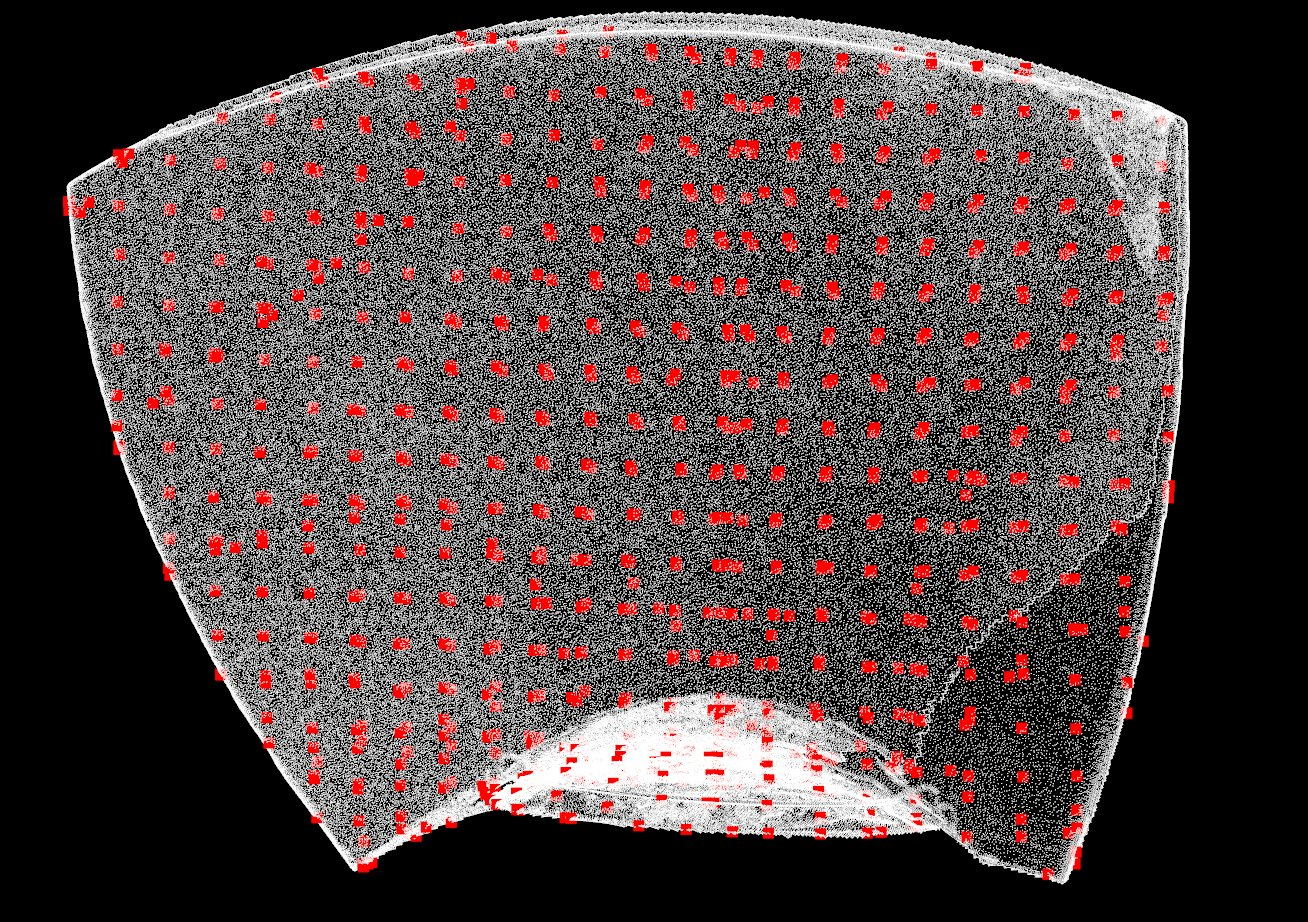
\includegraphics[width=0.95\columnwidth]{figs/localizacao/pa_key}
   \caption{Pontos de interesses com descritores associados no modelo da pá}
   \label{fig::pa_key}
\end{figure}

Uma vez que os pontos de interesse do modelo e seus descritores são extraídos, é
possível armazená-los para evitar o seu processamento  durante cada nova
calibração. Utilizando-se a estratérgia de
\textit{Correspondence Grouping} e o algoritmo \textit{Hough Voting}
\cite{Tombari2010a}, a nuvem de pontos aquisitada em campo terá também seus
pontos de interesse extraídos e um descritor associado para cada ponto. A
seguir, os descritores de ambas as nuvens, cena e modelo, são comparados afim de
se encontrar correpondentes em cada conjunto. Se um número suficiente de
correspondências é encontrado, o objeto é então detectado e localizado na
imagem. É importante ressaltar que essa técnica pode gerar falsos positivos. A
figura \ref{fig::correspondence} ilustra a implementação do algoritmo com 
dados sintéticos de uma cena, utilizando-se porém o modelo real da pá. O modelo
da pá está representado em amarelo, a pá identificada na cena em vermelho e as correspondências
conectadas pelas setas verdes.
Como próximos passos é necessário a utilização de dados reais para validação do
algoritmo e também a utilização de diferentes descritores, uma vez que apenas os
descritores do tipo SHOT foram testados.

\begin{figure}[h!]
   \centering
   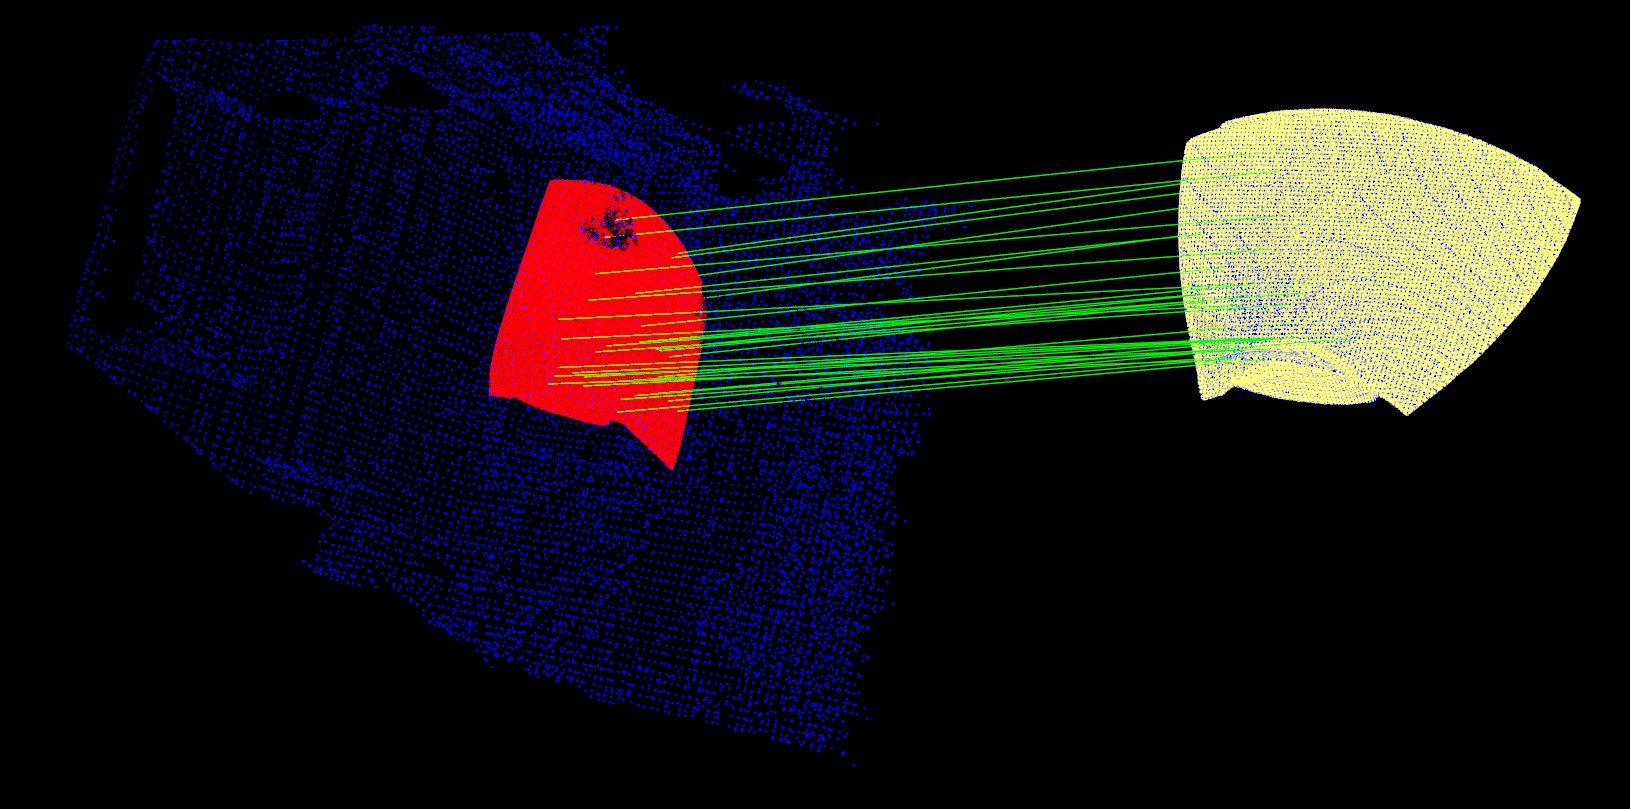
\includegraphics[width=0.99\columnwidth]{figs/localizacao/correspondence}
   \caption{Identificação e localização de uma pá utilizando
   \textit{Correspondence Grouping}}
   \label{fig::correspondence}
\end{figure}



